\documentclass[tikz]{standalone} 

\usepackage{newtxtext,newtxmath}

% mytikzset

\usetikzlibrary{positioning,arrows,shapes}
\usetikzlibrary{decorations.pathmorphing}
\usetikzlibrary{decorations.markings}

\tikzset{
  vector/.style={thick,double,draw=black, postaction={decorate},
    decoration={markings,mark=at position .6 with {\arrow[black,scale=0.4]{triangle 45}}}},
  axial/.style={thick,double,densely dashed,draw=black, postaction={decorate},
    decoration={markings,mark=at position .6 with {\arrow[black,scale=0.4]{triangle 45}}}},
  gluon/.style={decorate, draw=black,
    decoration={coil,aspect=0.3,segment length=5pt,amplitude=3pt}},
  pseudo/.style={thick, dashed, draw=black, postaction={decorate},
    decoration={markings,mark=at position .6 with {\arrow[red,scale=0.5]{triangle 45}}}},
  scalar/.style={thick,draw=black, postaction={decorate},
    decoration={markings,mark=at position .6 with {\arrow[black,scale=0.5]{triangle 45}}}}%,
  % pomeron/.style={thick,draw=black, postaction={decorate},
  % decoration={zigzag,segment length=4,amplitude=.9}}
}

\definecolor{myGreen}{RGB}{0,127,0}

\begin{document}
\nopagecolor
  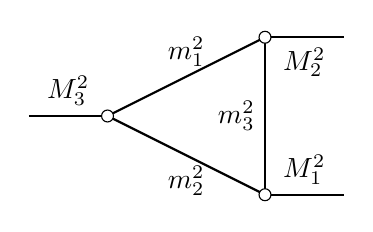
\begin{tikzpicture}[node distance=0.6cm and 0.9cm, baseline=1cm]
    \draw[thick]  (0,0) -- node[above] {$M_3^2$} (1,0);
    \draw[thick]  (1,0) -- node[above] {$m_1^2$} (3,1);
    \draw[thick]  (1,0) -- node[below] {$m_2^2$} (3,-1);
    \draw[thick]  (3,-1) -- node[left] {$m_3^2$} (3,1);
    \draw[thick]  (3,-1) -- node[above] {$M_1^2$} (4,-1);
    \draw[thick]  (3,1) -- node[below] {$M_2^2$} (4,1);

    \draw[black, fill=white] (1,0) circle (0.5ex);
    \draw[black, fill=white] (3,1) circle (0.5ex);
    \draw[black, fill=white] (3,-1) circle (0.5ex);
  \end{tikzpicture}
\end{document}
